\chapter{Solution}
\minitoc

The main goal of this solution is to develop a recommendation system for an e-commerce platform. 
In this context, users are referred to as customers or buyers ( representing individuals interacting with the platform which can be through a website or an app ), 
while products are referred to as items ( representing the goods offered for sale ).

To operate all the stages of the recommendation pipeline and the system components, 
a lot of infrastructure and DevOps work is required, from data ingestion to the deployment of the components.
The following sections will explain the system components and the deployment and technologies used in each stage of the recommendation pipeline.

TODO maybe we have to create our own custom graph to add caching, API gateway, and automation and DevOps components with our own infrastructure 

\begin{figure}[H]
    \centering
    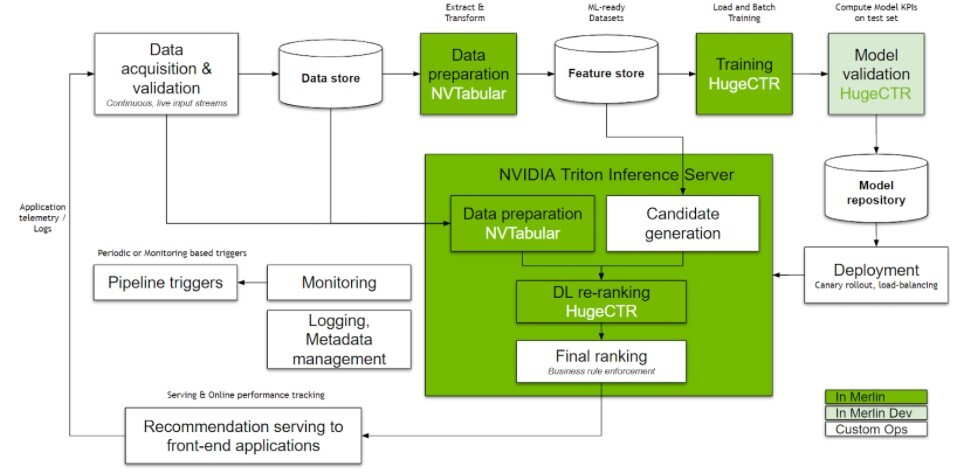
\includegraphics[width=1\textwidth]{assets/components.jpeg}
    \caption[System Components]{System Components \cite{NvidiaRecSysBestPractices}}
\end{figure}


The system components can be divided into the following categories:
\begin{itemize}
    \item API gateway
    \item Storage Components
    \item Recommendation Pipeline
    \item Caching Layer
    \item Automation and DevOps
\end{itemize}

Each component is explained in the following sections.

\section{API Gateway}

The API gateway, a RESTful API, is the entry point for the recommendation system.
It is responsible for handling all the requests and responses from the customers.
The main two functionalities of the API gateway are data ingestion and getting recommendations for a customer.

In addition to these functionalities, the API gateway is also responsible for authenticating and authorizing the requests.

\subsection{Data Ingestion Endpoints}

To handle the data ingestion, the API gateway exposes the following endpoints:
\begin{itemize}
    \item Create, Read, Update, Delete customers
    \item Create, Read, Update, Delete products
    \item Adding interactions between customers and products
\end{itemize}

Such endpoints interact mainly with the storage components to store the data.

\subsection{Recommendation Endpoints}

To get recommendations for a customer, the API gateway exposes the following endpoint:
\begin{itemize}
    \item Get recommendations for a customer
    \item Get similar products to a product
\end{itemize}

Those endpoints interact mainly with the recommendation pipeline and the caching layer to get the recommendations.

The first endpoint queries the caching layer to get the recommendations, and if the offline recommendations are not found in the caching layer, 
the API gateway queries the recommendation pipeline to get online recommendations, and then stores the recommendations in the caching layer and returns them to the customer.

In the second endpoint, the API gateway queries the feature store to get the embeddings of the product and then executes an Approximate Nearest Neighbor (ANN) search to get similar products.

\section{Storage Components}

The storage components are responsible for storing the data in different formats and stages, in addition to the models used in the recommendation system.
There are four main storage components in the system:

\begin{itemize}
    \item Main Database
    \begin{displayquote}
        The main database is an SQL database that stores the customers, products, and
         interactions data. In this project, a PostgreSQL\cite{Postgres} instance 
         deployed using AWS RDS \footnote{Amazon Web Services Relational Database Service \cite{AwsRDS}}
         is used as the main database. 
         But in a bigger production environment, a distributed Data Warehouse such as 
         Amazon Redshift\cite{AwsRedshift} or Google BigQuery\cite{GoogleBigQuery} can be used.
    \end{displayquote}
    \item Feature Store
    \begin{displayquote}
        The feature store is a storage system that stores data in a format optimized for machine learning models.\cite{NvidiaFeatureStores}
        It also stores the embedding tables of the customers 
        and products, in addition to any other categorical features.
        This project uses FEAST \cite{feast} as the feature store, which supports using a Redis\cite{Redis} cluster as an Online store, the Redis cluster is deployed using AWS ElastiCache\cite{AwsElastiCache}.
    \end{displayquote}

    \item Model Store
    \item Results Store
\end{itemize}

\section{Recommendation Pipeline}

* embedding store?
* choosing a ranking model and explaining it

\subsection{Candidate Generation}

\cite{NvidiaFeatureStores} READ THIS ! 

\subsubsection{Two Tower Model (Offline Retrieval)}

\subsubsection{ANN (Online Retrieval)}

\subsection{Rule Based Filtering (Filtering)}
* Explaining the E-commerce business logic
TODO 



\subsection{Deep Learning Ranking Model (Scoring Stage)}

* choosing a ranking model and explaining it
* storing model parameters?

\subsection{E-commerce ordering logic (Ordering Stage)}

* add additional business logic like promoting items (sponsored items), write an equation for the final score ( maybe ranking score + 0.2 for sponsored items or put sponsored items on top of the list if they exceed a certain threshold score)


* 
* Components Deployment ( ECS or Kubernetes, SageMaker or Triton Inference Server, Redis or Memcached, which feature store )?

\section{Storing Results}

* Redis or any memory store

TODO

\section{Automation and DevOps}
